%!TEX root = ../main.tex

\chapter{Template features}\label{ch:feats}

This chapter is divided in two parts.
First, it describes the features that are specific to this template: localization, logos, PDF/A compliance, the PhD cover, and the options to customize the style of the document (Sections~\ref{sec:logos}--\ref{sec:custom}).
Then, it shows how the most common \LaTeX{} features look like in this template, starting from Section~\ref{sec:text}.


\section{Logos}\label{sec:logos}

By default, the template is using the new logo of the University of Padova.
If required by your department/school, you can switch to the old logo with the \texttt{oldlogo} option of the document class:
\begin{lstlisting}[language=TeX]
\documentclass[
    oldlogo,
]{unipd-thesis-modern}
\end{lstlisting}
The option switches all the logos used by the template at once: the logo on the cover, the seal in the background of the cover, and the seal on top of the PhD cover (Section~\ref{sec:phdcover}).
Below, the new logo of the University of Padova (right), used by default, and the old one (left), set by the \texttt{oldlogo} option.
For backward compatibility, the \verb|\useoldlogo| command of previous versions of the template (v1.3) still works, when used in the preamble.

\begin{center}
    \begin{tikzpicture}
        \node (old) at (0,0) {
\includegraphics[height=1.6cm]{template/universis.old}};
        \node (new) at (9.5,0) {
\includegraphics[height=1.6cm]{template/universis}};
        \draw[<-, thick, shorten <=4mm, shorten >=4mm] (old.east) -- node[above=1mm] {\texttt{oldlogo}} (new.west);
    \end{tikzpicture}
\end{center}




\section{Language localization}\label{sec:language}

This template supports localization in both \textbf{English} and \textbf{Italian}. By default, the template uses \textbf{English}.
To select a different language, use the option when loading the document class:

\begin{lstlisting}[language=TeX]
\documentclass[
    language=italian,
]{unipd-thesis-modern}
\end{lstlisting}

The selected language is passed to \texttt{babel}, which automatically localizes all standard \LaTeX{} elements, including chapter and section names, figure and table captions, the table of contents, bibliography titles, dates, and hyphenation rules.

In addition, the template localizes all custom text that is not handled by \texttt{babel}, such as \emph{Supervisor}, \emph{Co-supervisor}, \emph{Academic Year}, and \emph{Student ID}.\\

You can extend the template to support additional languages by creating a new localization file in the \texttt{template/} directory. The file name must match one of the languages supported by \texttt{babel} (for example, \texttt{french.tex} or \texttt{german.tex}).

Inside this file, define all language-specific macros used by the template, following the structure of the existing localization files (e.g., \texttt{english.tex} and \texttt{italian.tex}). Once the file has been added, the new language can be selected through the \texttt{language} option of the document class.




\section{PDF/A compliance}\label{sec:pdfa}

The University submission system requires the final manuscript to be provided as a PDF/A compliant document.
For this reason, this template enforces the \textbf{PDF/A-2b} standard at compilation time through the \verb|pdfx| package.

To verify compliance of the generated PDF, you may use an online validation service such as
\href{https://www.pdfforge.org/online/en/validate-pdfa}{pdfforge PDF/A validator}.\\

\noindent
\textbf{Compiler compatibility.}
As of 2026, some incompatibilities have been observed between PDF/A generation and the \verb|pdfLaTeX| compiler when using the Palatino text font package \verb|newpxtext| adopted by this template.
These issues may result in PDF/A validation errors related to embedded font consistency.

For this reason, the recommended compiler for this template is \textbf{LuaLaTeX}, which provides full compatibility with the default font configuration and generally produces valid PDF/A output without requiring further modifications.

If LuaLaTeX is not available, the following alternatives may be considered:

\begin{itemize}
    \item \textbf{Use pdfLaTeX with \texttt{mathpazo}.}  
    This requires editing the template class file and replacing \verb|newpxtext| with \verb|mathpazo| (already included as a commented alternative). This configuration is PDF/A compliant, although it produces slightly different text and mathematical typography.

    \item \textbf{Post-process the generated PDF.}  
    If your document relies on packages or graphical features that interfere with PDF/A compliance (for instance transparency effects or unsupported font configurations), you may generate a standard PDF and convert it afterward using an external PDF/A conversion service such as
    \href{https://www.pdfforge.org/online/en/pdf-to-pdfa}{pdfforge PDF/A converter}.
\end{itemize}

The available PDF/A workflows are summarized in Table~\ref{tab:pdfa}.

\begin{table}[h!]
\small
\centering
\def\arraystretch{1.4}
\begin{tabular}{c|p{2.8cm}|c|c}\hline
\textbf{Option} & \textbf{Font package} & \textbf{pdfLaTeX} & \textbf{LuaLaTeX (recommended)} \\
\hline\hline
1 & \verb|newpxtext| 
& Known PDF/A compatibility issues 
& Works out of the box \\
\hline
2 & \verb|mathpazo| 
& Works out of the box 
& Works out of the box \\
\hline
3 & \multicolumn{3}{c}{Use external conversion to PDF/A on compiled document.}\\
\hline
\end{tabular}
\caption{\label{tab:pdfa}Available workflows for PDF/A-compliant document generation.}
\end{table}


\section{PhD cover}\label{sec:phdcover}

The PhD school requires a specific title page, following the \emph{facsimile frontespizio tesi PhD} provided by the school.
To use it instead of the default cover, enable the \texttt{phdcover} option of the document class:

\begin{lstlisting}[language=TeX]
\documentclass[
    phdcover,
]{unipd-thesis-modern}
\end{lstlisting}

The PhD cover uses the following fields, in addition to \verb|\title|, \verb|\author|, \verb|\advisor| and \verb|\coadvisor|:

\begin{lstlisting}[language=TeX]
\department{Department of Physics and Astronomy ``G. Galilei''}
\phdCourse{Physics}
\phdCurriculum{Theoretical Physics}  % optional
\phdSeries{XXXIX}
\phdCoordinator{Prof. Name Surname}
% optional, only for grants financed by external institutions:
\phdFunding{Thesis written with the financial contribution of ...}
\end{lstlisting}

Optional fields are omitted from the page when left empty, together with the space around them.
Fields spanning more lines (for instance, a long title or funding sentence) push the following elements down.

The labels follow the selected language (Section~\ref{sec:language}), and each of them can be overridden with \verb|\setphdlabel{<key>}{<text>}|, where the key is one of \texttt{course}, \texttt{curriculum}, \texttt{series}, \texttt{coordinator}, \texttt{supervisor}, \texttt{cosupervisor}, \texttt{student}.
For instance, to use the feminine form of the student label in Italian, add to the preamble:
\begin{lstlisting}[language=TeX]
\setphdlabel{student}{Dottoranda:}
\end{lstlisting}



\section{Stylistic customizations}\label{sec:custom}

The following options of the document class tweak the look of the document.
They are all independent of each other, and the style options are off by default:

\begin{lstlisting}[language=TeX]
\documentclass[
    textwidth=156mm, % width of the text block
    chapterskip=7mm, % space between chapter title and text
    boxedsections,   % section numbers inside a coloured box
    boxedcaptions,   % coloured square before caption labels
    thmtriangles,    % triangle markers in theorem headings
]{unipd-thesis-modern}
\end{lstlisting}

The \texttt{main.tex} of this demo enables some of them, so that you can see their effect in this document.

\subsection{Text width}

The \texttt{textwidth} option sets the width of the text block (\texttt{156mm} by default).
The horizontal margins are then computed automatically: a gutter of 10\,mm is added on the binding side, and the remaining space is split equally between the inner and outer margins.
For instance, on A4 paper, \texttt{textwidth=156mm} gives inner and outer margins of 32\,mm and 22\,mm, while \texttt{textwidth=150mm} gives 35\,mm and 25\,mm.
The chapter headings follow the margins automatically.

\subsection{Chapter spacing}

The \texttt{chapterskip} option sets the space between the title of a chapter and the text that follows.
It is measured from the baseline of the last line of the title to the top of the capital letters of the first line of text, so it is the same for titles spanning one or more lines.
The default is quite large (\texttt{27.5mm}), while a smaller value like \texttt{chapterskip=7mm} gives a more compact look, which might be preferred for shorter documents like a Bachelor thesis.

\subsection{Boxed sections}

With \texttt{boxedsections}, the section numbers are printed inside a coloured box.
Unnumbered sections (\verb|\section*|) are not affected.
Below, a section heading with the default style (left) and with the option (right):

\begin{center}
    \begin{tikzpicture}
        \draw[->, thick] (-1.5,0) -- node[above=1mm] {\texttt{boxedsections}} (1.5,0);
        \node[anchor=east, draw=black!25, rounded corners=2pt, inner sep=8pt] at (-1.8,0)
            {\normalfont\Large\bfseries 1.3\hspace{0.8em}Section title};
        \node[anchor=west, draw=black!25, rounded corners=2pt, inner sep=8pt] at (1.8,0)
            {\normalfont\Large\bfseries\colorbox{boxedColor}{\color{boxedTextColor}\kern0.15em 1.3\kern0.15em}\hspace{0.8em}Section title};
    \end{tikzpicture}
\end{center}

\subsection{Boxed captions}

With \texttt{boxedcaptions}, a small coloured square is printed before the label of every caption: figures, tables, code listings and algorithms (also those of the \texttt{algorithm2e} package).
Below, a caption with the default style (left) and with the option (right):

\begin{center}
    \begin{tikzpicture}
        \draw[->, thick] (-1.5,0) -- node[above=1mm] {\texttt{boxedcaptions}} (1.5,0);
        \node[anchor=east, draw=black!25, rounded corners=2pt, inner sep=8pt] at (-1.8,0)
            {\small\textbf{Figure 2.1:} A nice plot.};
        \node[anchor=west, draw=black!25, rounded corners=2pt, inner sep=8pt] at (1.8,0)
            {\small{\color{boxedColor}\rule{0.73em}{0.73em}}\hspace*{0.67em}\textbf{Figure 2.1:} A nice plot.};
    \end{tikzpicture}
\end{center}
You can see the effect on all the floating objects of this document, for instance Table~\ref{tab:pdfa}.

The colours of the boxes are \texttt{boxedColor} (by default, the main colour of the template, see Section~\ref{sec:color}) and \texttt{boxedTextColor} (the number inside the section box, white by default).
You can change them in the preamble, for instance with \verb|\colorlet{boxedColor}{orange}|.

\subsection{Theorem markers}

With \texttt{thmtriangles}, a small triangle is printed before the heading of theorem-like environments. Proofs keep the standard end-of-proof square.
The option loads the \texttt{amsthm} package, so you can define your environments with \verb|\newtheorem| as usual (see \texttt{custom-symbols.tex}).
Below, a proposition with its proof in the default style (left) and with the option (right):

\begin{center}
    \begin{tikzpicture}
        \draw[->, thick] (-1.2,0) -- node[above=1mm] {\texttt{thmtriangles}} (1.2,0);
        \node[anchor=east, draw=black!25, rounded corners=2pt, inner sep=8pt] at (-1.5,0)
            {\parbox{5.2cm}{\small\raggedright
                \textbf{Proposition 1.} \textit{The sum of two even numbers is even.}\par\smallskip
                \textit{Proof.} Let $2a$ and $2b$ be even. Then $2a+2b = 2(a+b)$.\hfill$\square$}};
        \node[anchor=west, draw=black!25, rounded corners=2pt, inner sep=8pt] at (1.5,0)
            {\parbox{5.2cm}{\small\raggedright
                \textcolor{thmMarkerColor}{$\blacktriangleright$}\nobreakspace\textbf{Proposition 1.} \textit{The sum of two even numbers is even.}\par\smallskip
                \textit{Proof.} Let $2a$ and $2b$ be even. Then $2a+2b = 2(a+b)$.\hfill$\square$}};
    \end{tikzpicture}
\end{center}

The marker is applied to the \texttt{plain}, \texttt{definition} and \texttt{remark} theorem styles, and its colour is \texttt{thmMarkerColor}.
Note that the template already defines an \texttt{example} box (Section~\ref{sec:boxes}), so pick a different name for an \emph{example} theorem environment.

\subsection{Colors}\label{sec:color}

The template is defined around color identifiers. \texttt{mainColor} is set to the classic red color of the UniPD color palette.
By default, the color of the rectangle in the Chapter headlines and the color of the box in the Part page are inherited from the main color,
\begin{lstlisting}[language={[latex]TeX}]
\colorlet{chapterColor}{mainColor}
\colorlet{partBoxColor}{mainColor}
\end{lstlisting}
which you can change by redefining the color inside the \texttt{.cls} template:
\begin{lstlisting}[language={[latex]TeX}]
\definecolor{chapterColor}{RGB}{255, 187, 0}
\end{lstlisting}

The options described above define some additional colours, all of which can be changed in the preamble with \verb|\colorlet|:
\begin{itemize}
    \item \texttt{boxedColor} and \texttt{boxedTextColor}, for the boxes of \texttt{boxedsections} and \texttt{boxedcaptions};
    \item \texttt{thmMarkerColor}, for the triangles of \texttt{thmtriangles};
    \item \texttt{sealColor}, for the seal on top of the PhD cover (Section~\ref{sec:phdcover}).
\end{itemize}




\section{Writing text}\label{sec:text}

I assume you already know how to use \LaTeX, so I won't write a lot.
Some \emph{words} are more important than others, so you might want to \emph{emphasize} them with the \verb|\emph| command.
On the other hand, you might wanna tell more about something without taking up a lot of space in the main text.
That's when you use footnotes\footnote{Just use the command \texttt{footnote}.}.

In a good scientific text, it is crucial to cite other people's work. If you say something important, make sure to \verb|\cite| it soon afterward \cite{10.1088/1367-2630/ad313e}. By the way, Ref.~\cite{10.1088/1367-2630/ad313e} is not saying anything useful for this purpose, so don't look at it. The bibliography entries are located in \texttt{refs.bib}.




\section{Math}

An equation might look like this $\mathcal{H}(\lambda) = A(t)\mathcal{H}_{A} + B(t)\mathcal{H}_{B}$, if inline. 
Otherwise, you might take more space:
\begin{equation*}
    \mathcal{H}(\lambda) = A(t)\mathcal{H}_{A} + B(t)\mathcal{H}_{B} + C(t)\mathcal{H}_{C} + ...
\end{equation*}

I will put here more math stuff with equations, just to make my point. Let $\ket{\psi(t)}$ be a quantum state that evolves in the time interval $[0,\tau]$. Its dynamics are described by the time-dependent Schrödinger equation.
$$i\ket{\dot\psi(t)} = \mathcal{H}(t)\ket{\psi(t)}$$
We use from now on the natural units $\hbar=1$. Let us introduce the basis of instantaneous eigenstates $\ket{n(t)}$ with eigenvalues $\epsilon_n(t)$:
\begin{equation}
    \label{eq:adth-eigenvalue}
    \mathcal{H}(t)\ket{n(t)} = \epsilon_n(t) \ket{n(t)}
\end{equation}
Since $\{\ket{n(t)}\}$ is a complete orthonormal set, $\ket{\psi(t)}$ can be expressed as a linear combination in that basis:
\begin{equation}
    \ket{\psi(t)} = \sum_n c_n(t) e^{i\theta_n(t)} \ket{n(t)}
\end{equation}
We have explicitly factorized the phase $\theta_n(t)=\int_0^t \epsilon_n(t')dt'$ from $c_n(t)$. This choice will be convenient in the following calculations, but it can be intuitively motivated straight away. 
It is known that an eigenstate picks up a phase $e^{-i\epsilon_n}$ when it evolves under a constant Hamiltonian. The $\theta_n(t)$ is a generalization of the picked-up phase, obtained by integrating it throughout the time interval in which the Hamiltonian evolves. It is known as the Berry phase.\\


To show the use of \verb|\underbrace{}|, we now write the Schrödinger equation in a rotating frame:
\begin{align}
    i\frac{d\ket{\tilde{\psi}}}{dt} &= i\left( \frac{dU^\dag}{dt}\ket{\psi} + U^\dag \frac{d\ket{\psi}}{dt} \right) = \nonumber\\
    &= i\dot\lambda \partial_\lambda U^\dag \cdot U\ket{\tilde{\psi}} + U^\dag\mathcal{H}\cdot U\ket{\tilde{\psi}} =\nonumber\\
    & \equiv \underbrace{\left( \tilde{\mathcal{H}} - \dot\lambda \tilde{\mathcal{A}}_\lambda \right)}_{\mathcal{H}_{rot}}\ket{\tilde{\psi}} \label{eq:schr-movingframe}
\end{align}

Just a suggestion: define recurrent symbols in \texttt{custom-symbols.tex}. For instance, typing \verb|\hamCD| to print $\hamCD$ is way more compact than typing
\begin{center}
    \verb|\mathcal{H}_{\mathrm{CD}}|
\end{center}
all the time...





\subsection{Theorem support}\label{sec:theorems}

You might input some theorem!

\begin{theorem}
Suppose that the spectrum of $\mathcal{H}(\lambda)$ has the ground state eigenvalue separated by a gap $\Delta(\lambda)=\epsilon_1(\lambda)-\epsilon_0(\lambda)\ >0$ from the rest of the spectrum, and that $\mathcal{H}$ is twice continuously differentiable. Assume that $\mathcal{H}$, $\partial_\lambda\mathcal{H}$ and $\partial^2_\lambda\mathcal{H}$ are bounded operators (an assumption that is always fulfilled in finite-dimensional spaces). Then
\begin{equation}
    \tau \gg \max\left(
        \max_\lambda \frac{\|\partial_\lambda\mathcal{H}(\lambda)\|}{\Delta^2(\lambda)},
        \max_\lambda \frac{\|\partial^2_\lambda\mathcal{H}(\lambda)\|}{\Delta^2(\lambda)}, 
        \max_\lambda \frac{\|\partial_\lambda\mathcal{H}(\lambda)\|^2}{\Delta^3(\lambda)}
    \right) .
\end{equation}
\end{theorem}








\section{Glossary}

In \texttt{docs/glossary.tex}, one might introduce acronyms that are printed in the table at the end of the document. The syntax is simple:

\begin{center}
    \verb|\newacronym{acronym-label}{EAT}{Extended Acronym Text}|
\end{center}

To reference the acronym, use the command \verb|\gls|. 
In the previous example, the command \verb|\gls{acronym-label}| will print:
\begin{itemize}
    \item \gls{acronym-label}, if the acronym has not been used before.
    \item \gls{acronym-label}, if the acronym has already been used in the text.
    \item Here, \gls{acronym-label} has been called for the third time!
\end{itemize}

It is possible to reset the counter for all the acronyms with \verb|\glsresetall|, or to reset the counter for a specific acronym with \verb|\glsreset{acronym-label}|.

\section{References and floating objects}

Using the \verb|\ref| command, you might reference labeled objects.
Chapter~\ref{ch:feats} is the only useful chapter of this template.
All the others, in Part~\ref{prt:filler}, are just filled with \texttt{lipsum} text.
The appendices are referenced with letters: for instance Appendix~\ref{ax:demo}.\\

When referencing equations, it is recommended to use \verb|\eqref| instead. 
For instance, Eq.~\eqref{eq:adth-eigenvalue} is clearly understood by any physics undergraduate!\\

Tables in \LaTeX are quite nice! Take a look at Table~\ref{tab:demo}.\\

\begin{table}[h]
\centering
\begin{tabular}{c|c|cc|cc}
    &\multirow{2}{*}{UA}&\multicolumn{2}{c|}{CD}&\multicolumn{2}{c}{FE}\\
    &&$\ell=1$&$\ell=2$&$\ell=1$&$\ell=2$\\\hline
    $f(\tau) \;[10^{-2}]$&1.5793&7.4970&17.039&7.5554&17.162\\
    $m(\tau)$&0.50107&0.69264&0.80038&0.69354&0.80143\\
    \hline
\end{tabular}
\caption{\label{tab:demo}Fidelity and energy merit resulting from an annealing simulation.}
\end{table}



Another kind of floating object are, of course, figures! To keep it simple, look at Figure~\ref{fig:demo}.\\

\begin{figure}
    \centering
    \includegraphics[height=6cm]{example-image-a}
    \caption{Simple example of floating image demo.}
    \label{fig:demo}
\end{figure}


As for plots, I recommend you save them in PDF format (Figure~\ref{fig:demo-plot}).

\begin{figure}
    \centering
    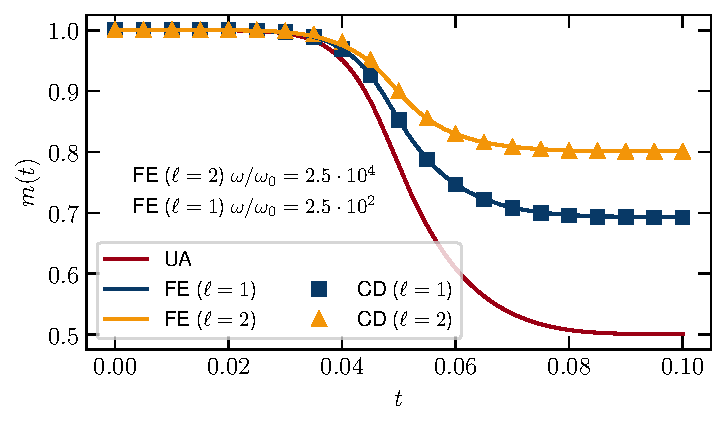
\includegraphics[height=7cm]{img/demo-plot.pdf}
    \caption{Simple example of plot saved in PDF and imported in the document. This ensures correctly vectorized images.}
    \label{fig:demo-plot}
\end{figure}


\lipsum[1-5]






\section{Drawing with tikz}

When you get skilled, you might want to create drawings in \texttt{tikz}, like in Figure~\ref{fig:demo-max-cut}.
You can make equations with drawings,
% note: this is an equation with drawings\
%
% Gradient Info
\tikzset {_2wjvdlgsv/.code = {\pgfsetadditionalshadetransform{ \pgftransformshift{\pgfpoint{0 bp } { 0 bp }  }  \pgftransformrotate{-45 }  \pgftransformscale{2 }  }}}
\pgfdeclarehorizontalshading{_189nw8o3l}{150bp}{rgb(0bp)=(0.03,0.22,0.4);
rgb(37.5bp)=(0.03,0.22,0.4);
rgb(43.86904580252511bp)=(0.03,0.22,0.4);
rgb(62.5bp)=(0.05,0.36,0.63);
rgb(100bp)=(0.05,0.36,0.63)}
\tikzset{every picture/.style={line width=0.75pt}} %set default line width to 0.75pt         
%
%
\begin{equation}
\label{eq:demo-tikz-eq}
\begin{tikzpicture}[baseline={([yshift=-.5ex]current bounding box.center)},x=0.75pt,y=0.75pt,yscale=-1,xscale=1]

%Shape: Square [id:dp9442510713449753] 
\draw  [draw opacity=0][shading=_189nw8o3l,_2wjvdlgsv] (20,20) -- (70,20) -- (70,70) -- (20,70) -- cycle ;

% Text Node
\draw (8,9) node [anchor=north west][inner sep=0.75pt]    {$\textcolor{red}{y}$};
% Text Node
\draw (72,9) node [anchor=north west][inner sep=0.75pt]    {$z$};
% Text Node
\draw (8,72) node [anchor=north west][inner sep=0.75pt]    {$z$};
% Text Node
\draw (72,72) node [anchor=north west][inner sep=0.75pt]    {$z$};
% Text Node
\draw (22,24) node [anchor=north west][inner sep=0.75pt]  [font=\footnotesize,color={rgb, 255:red, 255; green, 255; blue, 255 }  ,opacity=1 ] [align=left] {a};
% Text Node
\draw (60,21) node [anchor=north west][inner sep=0.75pt]  [font=\footnotesize,color={rgb, 255:red, 255; green, 255; blue, 255 }  ,opacity=1 ] [align=left] {b};
% Text Node
\draw (60,59) node [anchor=north west][inner sep=0.75pt]  [font=\footnotesize,color={rgb, 255:red, 255; green, 255; blue, 255 }  ,opacity=1 ] [align=left] {c};
% Text Node
\draw (22,56) node [anchor=north west][inner sep=0.75pt]  [font=\footnotesize,color={rgb, 255:red, 255; green, 255; blue, 255 }  ,opacity=1 ] [align=left] {d};

\end{tikzpicture}
\equiv \textcolor{red}{\hat\sigma_y^{(a)}}\otimes\hat\sigma_z^{(b)}\otimes\hat\sigma_z^{(c)}\otimes\hat\sigma_z^{(d)}
\end{equation}
or tables with drawings, like in Table~\ref{tab:demo-draw}... 

\lipsum[1-2]



\begin{figure}
    \centering
    

\tikzset{every picture/.style={line width=0.75pt}} %set default line width to 0.75pt        

\begin{tikzpicture}[x=0.75pt,y=0.75pt,yscale=-1,xscale=1]
%uncomment if require: \path (0,159); %set diagram left start at 0, and has height of 159

%Straight Lines [id:da11964796995332005] 
\draw    (158.5,73.5) -- (259.5,37.5) ;
%Straight Lines [id:da15972910359553594] 
\draw [color={rgb, 255:red, 255; green, 0; blue, 0 }  ,draw opacity=1 ][line width=1.5]    (158.5,73.5) -- (168,133.5) ;
%Straight Lines [id:da2798044521653187] 
\draw [color={rgb, 255:red, 255; green, 0; blue, 0 }  ,draw opacity=1 ][line width=1.5]    (259.5,37.5) -- (198.5,20.5) ;
%Straight Lines [id:da7169631782552711] 
\draw [color={rgb, 255:red, 255; green, 0; blue, 0 }  ,draw opacity=1 ][line width=1.5]    (158.5,73.5) -- (198.5,20.5) ;
%Straight Lines [id:da026668841375865227] 
\draw [color={rgb, 255:red, 255; green, 0; blue, 0 }  ,draw opacity=1 ][line width=1.5]    (168,133.5) -- (259.5,37.5) ;
%Straight Lines [id:da10247267579193942] 
\draw [color={rgb, 255:red, 255; green, 0; blue, 0 }  ,draw opacity=1 ][line width=1.5]    (158.5,73.5) -- (42,59.5) ;
%Straight Lines [id:da6325731661518962] 
\draw [color={rgb, 255:red, 255; green, 0; blue, 0 }  ,draw opacity=1 ][line width=1.5]    (168,133.5) -- (72,114) ;
%Straight Lines [id:da6714305559976217] 
\draw [color={rgb, 255:red, 255; green, 0; blue, 0 }  ,draw opacity=1 ][line width=1.5]    (72,114) -- (42,59.5) ;
%Shape: Ellipse [id:dp9445310521915122] 
\draw  [fill={rgb, 255:red, 74; green, 144; blue, 226 }  ,fill opacity=1 ] (246.5,37.5) .. controls (246.5,30.32) and (252.32,24.5) .. (259.5,24.5) .. controls (266.68,24.5) and (272.5,30.32) .. (272.5,37.5) .. controls (272.5,44.68) and (266.68,50.5) .. (259.5,50.5) .. controls (252.32,50.5) and (246.5,44.68) .. (246.5,37.5) -- cycle ;
%Shape: Ellipse [id:dp5491993786197626] 
\draw  [fill={rgb, 255:red, 255; green, 255; blue, 255 }  ,fill opacity=1 ] (29,59.5) .. controls (29,52.32) and (34.82,46.5) .. (42,46.5) .. controls (49.18,46.5) and (55,52.32) .. (55,59.5) .. controls (55,66.68) and (49.18,72.5) .. (42,72.5) .. controls (34.82,72.5) and (29,66.68) .. (29,59.5) -- cycle ;
%Curve Lines [id:da8424711661169174] 
\draw [line width=1.5]  [dash pattern={on 3.75pt off 1.5pt}]  (34.5,91.5) .. controls (68,94) and (64.56,99.23) .. (95.5,76) .. controls (126.44,52.77) and (148,51.5) .. (174,53) .. controls (200,54.5) and (248,-13.5) .. (281.92,24.92) .. controls (315.83,63.33) and (185.58,99.58) .. (163.25,103.5) .. controls (140.92,107.42) and (111.42,122.92) .. (107.92,141.42) ;
%Shape: Ellipse [id:dp8814510692429732] 
\draw  [fill={rgb, 255:red, 255; green, 255; blue, 255 }  ,fill opacity=1 ] (337,52.5) .. controls (337,46.98) and (341.48,42.5) .. (347,42.5) .. controls (352.52,42.5) and (357,46.98) .. (357,52.5) .. controls (357,58.02) and (352.52,62.5) .. (347,62.5) .. controls (341.48,62.5) and (337,58.02) .. (337,52.5) -- cycle ;
%Shape: Ellipse [id:dp47339460639922903] 
\draw  [color={rgb, 255:red, 0; green, 0; blue, 0 }  ,draw opacity=1 ][fill={rgb, 255:red, 74; green, 144; blue, 226 }  ,fill opacity=1 ] (337,82.5) .. controls (337,76.98) and (341.48,72.5) .. (347,72.5) .. controls (352.52,72.5) and (357,76.98) .. (357,82.5) .. controls (357,88.02) and (352.52,92.5) .. (347,92.5) .. controls (341.48,92.5) and (337,88.02) .. (337,82.5) -- cycle ;
%Straight Lines [id:da23538055750108888] 
\draw [color={rgb, 255:red, 255; green, 0; blue, 0 }  ,draw opacity=1 ][line width=1.5]    (359.92,113) -- (334,113) ;
\draw [color={rgb, 255:red, 0; green, 0; blue, 0 }  ,draw opacity=1 ][line width=1.0]    (359.92,133) -- (334,133) ;
%Shape: Ellipse [id:dp4410323283239628] 
\draw  [fill={rgb, 255:red, 255; green, 255; blue, 255 }  ,fill opacity=1 ] (185.5,20.5) .. controls (185.5,13.32) and (191.32,7.5) .. (198.5,7.5) .. controls (205.68,7.5) and (211.5,13.32) .. (211.5,20.5) .. controls (211.5,27.68) and (205.68,33.5) .. (198.5,33.5) .. controls (191.32,33.5) and (185.5,27.68) .. (185.5,20.5) -- cycle ;
%Shape: Ellipse [id:dp23920294173784062] 
\draw  [fill={rgb, 255:red, 74; green, 144; blue, 226 }  ,fill opacity=1 ] (145.5,73.5) .. controls (145.5,66.32) and (151.32,60.5) .. (158.5,60.5) .. controls (165.68,60.5) and (171.5,66.32) .. (171.5,73.5) .. controls (171.5,80.68) and (165.68,86.5) .. (158.5,86.5) .. controls (151.32,86.5) and (145.5,80.68) .. (145.5,73.5) -- cycle ;
%Shape: Ellipse [id:dp6646352421974419] 
\draw  [fill={rgb, 255:red, 255; green, 255; blue, 255 }  ,fill opacity=1 ] (155,133.5) .. controls (155,126.32) and (160.82,120.5) .. (168,120.5) .. controls (175.18,120.5) and (181,126.32) .. (181,133.5) .. controls (181,140.68) and (175.18,146.5) .. (168,146.5) .. controls (160.82,146.5) and (155,140.68) .. (155,133.5) -- cycle ;
%Shape: Ellipse [id:dp5494896623298657] 
\draw  [fill={rgb, 255:red, 74; green, 144; blue, 226 }  ,fill opacity=1 ] (59,114) .. controls (59,106.82) and (64.82,101) .. (72,101) .. controls (79.18,101) and (85,106.82) .. (85,114) .. controls (85,121.18) and (79.18,127) .. (72,127) .. controls (64.82,127) and (59,121.18) .. (59,114) -- cycle ;

% Text Node
\draw (31,50.9) node [anchor=north west][inner sep=0.75pt]  [font=\normalsize]  {$V_{3}$};
% Text Node
\draw (360,50) node [anchor=north west][inner sep=0.75pt]  [font=\small]  {$\in U$};
% Text Node
\draw (360,72) node [anchor=north west][inner sep=0.75pt]  [font=\small]  {$\in \overline{U}$};
% Text Node
\draw (366.5,104.5) node [anchor=north west][inner sep=0.75pt]  [font=\small] [align=left] {cutted edges};
\draw (366.5,124.5) node [anchor=north west][inner sep=0.75pt]  [font=\small] [align=left] {uncutted edges};
% Text Node
\draw (187,11.4) node [anchor=north west][inner sep=0.75pt]  [font=\normalsize]  {$V_{5}$};
% Text Node
\draw (249,29.4) node [anchor=north west][inner sep=0.75pt]  [font=\normalsize,color={rgb, 255:red, 255; green, 255; blue, 255 }  ,opacity=1 ]  {$V_{6}$};
% Text Node
\draw (148,65.4) node [anchor=north west][inner sep=0.75pt]  [font=\normalsize,color={rgb, 255:red, 255; green, 255; blue, 255 }  ,opacity=1 ]  {$V_{4}$};
% Text Node
\draw (157,124.9) node [anchor=north west][inner sep=0.75pt]  [font=\normalsize]  {$V_{1}$};
% Text Node
\draw (61.5,105.9) node [anchor=north west][inner sep=0.75pt]  [font=\normalsize,color={rgb, 255:red, 255; green, 255; blue, 255 }  ,opacity=1 ]  {$V_{2}$};


\end{tikzpicture}

    \caption{An example of Maximum Cut problem. The dashed line cuts the seven edges that are highlighted in red. Consequently, the vertices are marked with different colors to indicate their belonging to partition $U$ or $\bar{U}$.}
    \label{fig:demo-max-cut}
\end{figure}



\begin{table}
\centering
\begin{tblr}{colspec={Q[c,h]cccc},stretch=0,rowsep=6pt}
\hline
spin indexing&N&label&sign of $J_k$&$\theta$\\\hline
\SetCell[r=3]{m} \scalebox{0.6}{

% Gradient Info
  
\tikzset {_q6d1jly0c/.code = {\pgfsetadditionalshadetransform{ \pgftransformshift{\pgfpoint{-7.5 bp } { 0 bp }  }  \pgftransformrotate{-225 }  \pgftransformscale{2 }  }}}
\pgfdeclarehorizontalshading{_0bsmz13ng}{150bp}{rgb(0bp)=(0.03,0.22,0.4);
rgb(37.5bp)=(0.03,0.22,0.4);
rgb(62.5bp)=(0,0.29,0.51);
rgb(100bp)=(0,0.29,0.51)}

% Gradient Info
  
\tikzset {_uvoxzm524/.code = {\pgfsetadditionalshadetransform{ \pgftransformshift{\pgfpoint{-7.5 bp } { 0 bp }  }  \pgftransformrotate{-225 }  \pgftransformscale{2 }  }}}
\pgfdeclarehorizontalshading{_fyest5jbo}{150bp}{rgb(0bp)=(0.03,0.22,0.4);
rgb(37.5bp)=(0.03,0.22,0.4);
rgb(62.5bp)=(0,0.29,0.51);
rgb(100bp)=(0,0.29,0.51)}

% Gradient Info
  
\tikzset {_py27uv7b1/.code = {\pgfsetadditionalshadetransform{ \pgftransformshift{\pgfpoint{-7.5 bp } { 0 bp }  }  \pgftransformrotate{-225 }  \pgftransformscale{2 }  }}}
\pgfdeclarehorizontalshading{_e66njv4ua}{150bp}{rgb(0bp)=(0.03,0.22,0.4);
rgb(37.5bp)=(0.03,0.22,0.4);
rgb(62.5bp)=(0,0.29,0.51);
rgb(100bp)=(0,0.29,0.51)}
\tikzset{every picture/.style={line width=0.75pt}} %set default line width to 0.75pt        


\begin{tikzpicture}[x=0.75pt,y=0.75pt,yscale=-1,xscale=1]
%uncomment if require: \path (0,141); %set diagram left start at 0, and has height of 141

%Shape: Square [id:dp40205531904810266] 
\draw  [draw opacity=0][shading=_0bsmz13ng,_q6d1jly0c] (120.31,35) -- (155.66,70.35) -- (120.31,105.71) -- (84.95,70.35) -- cycle ;
%Shape: Circle [id:dp6654608173556106] 
\draw   (113.24,13.78) .. controls (117.14,9.88) and (123.47,9.88) .. (127.38,13.78) .. controls (131.28,17.69) and (131.28,24.02) .. (127.38,27.92) .. controls (123.47,31.83) and (117.14,31.83) .. (113.24,27.92) .. controls (109.33,24.02) and (109.33,17.69) .. (113.24,13.78) -- cycle ;
%Shape: Circle [id:dp06811511385885272] 
\draw   (162.74,63.28) .. controls (166.64,59.37) and (172.97,59.37) .. (176.88,63.28) .. controls (180.78,67.19) and (180.78,73.52) .. (176.88,77.42) .. controls (172.97,81.33) and (166.64,81.33) .. (162.74,77.42) .. controls (158.83,73.52) and (158.83,67.19) .. (162.74,63.28) -- cycle ;
%Shape: Circle [id:dp866496050161264] 
\draw   (212.23,112.78) .. controls (216.14,108.87) and (222.47,108.87) .. (226.37,112.78) .. controls (230.28,116.68) and (230.28,123.01) .. (226.37,126.92) .. controls (222.47,130.82) and (216.14,130.82) .. (212.23,126.92) .. controls (208.33,123.01) and (208.33,116.68) .. (212.23,112.78) -- cycle ;
%Shape: Circle [id:dp8486257980974814] 
\draw   (63.74,63.28) .. controls (67.65,59.37) and (73.98,59.37) .. (77.88,63.28) .. controls (81.79,67.19) and (81.79,73.52) .. (77.88,77.42) .. controls (73.98,81.33) and (67.65,81.33) .. (63.74,77.42) .. controls (59.83,73.52) and (59.83,67.19) .. (63.74,63.28) -- cycle ;
%Shape: Circle [id:dp6621158362166136] 
\draw   (113.24,112.78) .. controls (117.14,108.87) and (123.47,108.87) .. (127.38,112.78) .. controls (131.28,116.68) and (131.28,123.01) .. (127.38,126.92) .. controls (123.47,130.82) and (117.14,130.82) .. (113.24,126.92) .. controls (109.33,123.01) and (109.33,116.68) .. (113.24,112.78) -- cycle ;
%Shape: Circle [id:dp9693194383410402] 
\draw   (14.24,112.78) .. controls (18.15,108.87) and (24.48,108.87) .. (28.38,112.78) .. controls (32.29,116.68) and (32.29,123.01) .. (28.38,126.92) .. controls (24.48,130.82) and (18.15,130.82) .. (14.24,126.92) .. controls (10.34,123.01) and (10.34,116.68) .. (14.24,112.78) -- cycle ;
%Shape: Right Triangle [id:dp28578880257729367] 
\draw  [draw opacity=0][shading=_fyest5jbo,_uvoxzm524] (105.92,120.1) -- (35.71,120.6) -- (71.06,85.24) -- cycle ;
%Shape: Right Triangle [id:dp9982201862645094] 
\draw  [draw opacity=0][shading=_e66njv4ua,_py27uv7b1] (205.16,119.85) -- (134.45,119.85) -- (169.81,84.49) -- cycle ;

% Text Node
\draw (115,14) node [anchor=north west][inner sep=0.75pt]   [align=left] {1};
% Text Node
\draw (66,63) node [anchor=north west][inner sep=0.75pt]   [align=left] {2};
% Text Node
\draw (165,63) node [anchor=north west][inner sep=0.75pt]   [align=left] {3};
% Text Node
\draw (16,113) node [anchor=north west][inner sep=0.75pt]   [align=left] {4};
% Text Node
\draw (115,113) node [anchor=north west][inner sep=0.75pt]   [align=left] {5};
% Text Node
\draw (214,113) node [anchor=north west][inner sep=0.75pt]   [align=left] {6};

\end{tikzpicture}} & \SetCell[r=3]{m} 6 
    & LHZ6E & $[+,+,-,-,+,-]$ &0.0 \\\hline
&   & \textbf{LHZ6M} & $[-,-,-,+,-,+]$ & 0.3\\\hline
&   & LHZ6H & $[+,+,+,-,-,+]$ & 0.55\\\hline
\hspace{-3mm}\scalebox{0.6}{

% Gradient Info
  
\tikzset {_2xhcrefu0/.code = {\pgfsetadditionalshadetransform{ \pgftransformshift{\pgfpoint{-7.5 bp } { 0 bp }  }  \pgftransformrotate{-225 }  \pgftransformscale{2 }  }}}
\pgfdeclarehorizontalshading{_spn6ydpdw}{150bp}{rgb(0bp)=(0.03,0.22,0.4);
rgb(37.5bp)=(0.03,0.22,0.4);
rgb(62.5bp)=(0,0.29,0.51);
rgb(100bp)=(0,0.29,0.51)}

% Gradient Info
  
\tikzset {_kw0p3luhv/.code = {\pgfsetadditionalshadetransform{ \pgftransformshift{\pgfpoint{-7.5 bp } { 0 bp }  }  \pgftransformrotate{-225 }  \pgftransformscale{2 }  }}}
\pgfdeclarehorizontalshading{_zquv02ocj}{150bp}{rgb(0bp)=(0.03,0.22,0.4);
rgb(37.5bp)=(0.03,0.22,0.4);
rgb(62.5bp)=(0,0.29,0.51);
rgb(100bp)=(0,0.29,0.51)}

% Gradient Info
  
\tikzset {_5nlio4lhy/.code = {\pgfsetadditionalshadetransform{ \pgftransformshift{\pgfpoint{-7.5 bp } { 0 bp }  }  \pgftransformrotate{-225 }  \pgftransformscale{2 }  }}}
\pgfdeclarehorizontalshading{_0px9iulda}{150bp}{rgb(0bp)=(0.03,0.22,0.4);
rgb(37.5bp)=(0.03,0.22,0.4);
rgb(62.5bp)=(0,0.29,0.51);
rgb(100bp)=(0,0.29,0.51)}

% Gradient Info
  
\tikzset {_i9m56ow0g/.code = {\pgfsetadditionalshadetransform{ \pgftransformshift{\pgfpoint{-7.5 bp } { 0 bp }  }  \pgftransformrotate{-225 }  \pgftransformscale{2 }  }}}
\pgfdeclarehorizontalshading{_cp2s0duqo}{150bp}{rgb(0bp)=(0.03,0.22,0.4);
rgb(37.5bp)=(0.03,0.22,0.4);
rgb(62.5bp)=(0,0.29,0.51);
rgb(100bp)=(0,0.29,0.51)}

% Gradient Info
  
\tikzset {_i0ciopkoo/.code = {\pgfsetadditionalshadetransform{ \pgftransformshift{\pgfpoint{-7.5 bp } { 0 bp }  }  \pgftransformrotate{-225 }  \pgftransformscale{2 }  }}}
\pgfdeclarehorizontalshading{_pfe2kjcao}{150bp}{rgb(0bp)=(0.03,0.22,0.4);
rgb(37.5bp)=(0.03,0.22,0.4);
rgb(62.5bp)=(0,0.29,0.51);
rgb(100bp)=(0,0.29,0.51)}

% Gradient Info
  
\tikzset {_4zjqptm1s/.code = {\pgfsetadditionalshadetransform{ \pgftransformshift{\pgfpoint{-7.5 bp } { 0 bp }  }  \pgftransformrotate{-225 }  \pgftransformscale{2 }  }}}
\pgfdeclarehorizontalshading{_2wsugf3gc}{150bp}{rgb(0bp)=(0.03,0.22,0.4);
rgb(37.5bp)=(0.03,0.22,0.4);
rgb(62.5bp)=(0,0.29,0.51);
rgb(100bp)=(0,0.29,0.51)}
\tikzset{every picture/.style={line width=0.75pt}} %set default line width to 0.75pt        

\begin{tikzpicture}[x=0.75pt,y=0.75pt,yscale=-1,xscale=1]
%uncomment if require: \path (0,184); %set diagram left start at 0, and has height of 184

%Shape: Square [id:dp4646069098280107] 
\draw  [draw opacity=0][shading=_spn6ydpdw,_2xhcrefu0] (166.72,29.33) -- (202.08,64.68) -- (166.72,100.04) -- (131.36,64.68) -- cycle ;
%Shape: Circle [id:dp1768374451497594] 
\draw   (159.65,8.11) .. controls (163.55,4.21) and (169.89,4.21) .. (173.79,8.11) .. controls (177.7,12.02) and (177.7,18.35) .. (173.79,22.26) .. controls (169.89,26.16) and (163.55,26.16) .. (159.65,22.26) .. controls (155.74,18.35) and (155.74,12.02) .. (159.65,8.11) -- cycle ;
%Shape: Circle [id:dp9515478681131959] 
\draw   (209.15,57.61) .. controls (213.05,53.71) and (219.38,53.71) .. (223.29,57.61) .. controls (227.19,61.52) and (227.19,67.85) .. (223.29,71.75) .. controls (219.38,75.66) and (213.05,75.66) .. (209.15,71.75) .. controls (205.24,67.85) and (205.24,61.52) .. (209.15,57.61) -- cycle ;
%Shape: Circle [id:dp7756495234805515] 
\draw   (258.64,107.11) .. controls (262.55,103.2) and (268.88,103.2) .. (272.79,107.11) .. controls (276.69,111.01) and (276.69,117.35) .. (272.79,121.25) .. controls (268.88,125.16) and (262.55,125.16) .. (258.64,121.25) .. controls (254.74,117.35) and (254.74,111.01) .. (258.64,107.11) -- cycle ;
%Shape: Circle [id:dp2733517995597814] 
\draw   (110.15,57.61) .. controls (114.06,53.71) and (120.39,53.71) .. (124.29,57.61) .. controls (128.2,61.52) and (128.2,67.85) .. (124.29,71.75) .. controls (120.39,75.66) and (114.06,75.66) .. (110.15,71.75) .. controls (106.25,67.85) and (106.25,61.52) .. (110.15,57.61) -- cycle ;
%Shape: Circle [id:dp7014226103914162] 
\draw   (159.65,107.11) .. controls (163.55,103.2) and (169.89,103.2) .. (173.79,107.11) .. controls (177.7,111.01) and (177.7,117.35) .. (173.79,121.25) .. controls (169.89,125.16) and (163.55,125.16) .. (159.65,121.25) .. controls (155.74,117.35) and (155.74,111.01) .. (159.65,107.11) -- cycle ;
%Shape: Circle [id:dp07847046561305948] 
\draw   (60.65,107.11) .. controls (64.56,103.2) and (70.89,103.2) .. (74.8,107.11) .. controls (78.7,111.01) and (78.7,117.35) .. (74.8,121.25) .. controls (70.89,125.16) and (64.56,125.16) .. (60.65,121.25) .. controls (56.75,117.35) and (56.75,111.01) .. (60.65,107.11) -- cycle ;
%Shape: Right Triangle [id:dp18543834280062976] 
\draw  [draw opacity=0][shading=_zquv02ocj,_kw0p3luhv] (202.08,164.18) -- (131.36,164.18) -- (166.72,128.82) -- cycle ;
%Shape: Right Triangle [id:dp019748006978987376] 
\draw  [draw opacity=0][shading=_0px9iulda,_5nlio4lhy] (300.82,163.93) -- (230.61,164.43) -- (265.97,129.07) -- cycle ;
%Shape: Circle [id:dp3946162772039473] 
\draw   (209.15,156.61) .. controls (213.05,152.7) and (219.38,152.7) .. (223.29,156.61) .. controls (227.19,160.51) and (227.19,166.84) .. (223.29,170.75) .. controls (219.38,174.65) and (213.05,174.65) .. (209.15,170.75) .. controls (205.24,166.84) and (205.24,160.51) .. (209.15,156.61) -- cycle ;
%Shape: Circle [id:dp6620738247447955] 
\draw   (110.15,156.61) .. controls (114.06,152.7) and (120.39,152.7) .. (124.29,156.61) .. controls (128.2,160.51) and (128.2,166.84) .. (124.29,170.75) .. controls (120.39,174.65) and (114.06,174.65) .. (110.15,170.75) .. controls (106.25,166.84) and (106.25,160.51) .. (110.15,156.61) -- cycle ;
%Shape: Circle [id:dp027305429094700795] 
\draw   (11.16,156.61) .. controls (15.06,152.7) and (21.39,152.7) .. (25.3,156.61) .. controls (29.2,160.51) and (29.2,166.84) .. (25.3,170.75) .. controls (21.39,174.65) and (15.06,174.65) .. (11.16,170.75) .. controls (7.25,166.84) and (7.25,160.51) .. (11.16,156.61) -- cycle ;
%Shape: Circle [id:dp5838580222665838] 
\draw   (308.14,156.61) .. controls (312.05,152.7) and (318.38,152.7) .. (322.28,156.61) .. controls (326.19,160.51) and (326.19,166.84) .. (322.28,170.75) .. controls (318.38,174.65) and (312.05,174.65) .. (308.14,170.75) .. controls (304.24,166.84) and (304.24,160.51) .. (308.14,156.61) -- cycle ;
%Shape: Right Triangle [id:dp051990486144260606] 
\draw  [draw opacity=0][shading=_cp2s0duqo,_i9m56ow0g] (102.83,163.93) -- (32.62,164.43) -- (67.98,129.07) -- cycle ;
%Shape: Square [id:dp556944438890764] 
\draw  [draw opacity=0][shading=_pfe2kjcao,_i0ciopkoo] (216.22,78.82) -- (251.57,114.18) -- (216.22,149.53) -- (180.86,114.18) -- cycle ;
%Shape: Square [id:dp31466343787367357] 
\draw  [draw opacity=0][shading=_2wsugf3gc,_4zjqptm1s] (117.22,78.82) -- (152.58,114.18) -- (117.22,149.53) -- (81.87,114.18) -- cycle ;

% Text Node
\draw (162,8) node [anchor=north west][inner sep=0.75pt]   [align=left] {1};
% Text Node
\draw (112,58) node [anchor=north west][inner sep=0.75pt]   [align=left] {2};
% Text Node
\draw (211,58) node [anchor=north west][inner sep=0.75pt]   [align=left] {3};
% Text Node
\draw (62,107) node [anchor=north west][inner sep=0.75pt]   [align=left] {4};
% Text Node
\draw (162,107) node [anchor=north west][inner sep=0.75pt]   [align=left] {5};
% Text Node
\draw (260,107) node [anchor=north west][inner sep=0.75pt]   [align=left] {6};
% Text Node
\draw (13,157) node [anchor=north west][inner sep=0.75pt]   [align=left] {7};
% Text Node
\draw (112,157) node [anchor=north west][inner sep=0.75pt]   [align=left] {8};
% Text Node
\draw (211,157) node [anchor=north west][inner sep=0.75pt]   [align=left] {9};
% Text Node
\draw (306,157) node [anchor=north west][inner sep=0.75pt]   [align=left] {10};


\end{tikzpicture}
} & 10 & LHZ10&\makecell{$[-,-,-,-,+$\\$\;\;+,+,-,-,-]$}&0.3\\
\hline
\end{tblr}
    \caption{\label{tab:demo-draw} Selected instances of LHZ models that are considered in the following analysis. The constraints are fixed to $C_l=-2$ and the magnitude of the local fields to $|J_k|=1$. The signs of $J_k$ that fully determine the instance are reported in the table, along with the label of the instance and its ``hardness'' $\theta$. The reference study case is LHZ6M.}
\end{table}

\section{Special boxes}\label{sec:boxes}

The template offers special environments for important text and comments...
\begin{info}
... like this one, \texttt{info}. Other special environments are \texttt{warning} and \texttt{example}, which differ from this only by the icon on the top left of the delimited area.
\end{info}
You can define your own custom environment via an \texttt{mdfdefinestyle}.
Have a look at \textit{template/extras.tex} for a reference.

\subsection{Code snippets}

The template integrates \texttt{listings} as the default environment for code snippets. You can define your own style in \textit{template/extras.tex}.

\begin{lstlisting}[language=Python]
def half(n: int): # comment
    return "the half is" + str(n//2)
\end{lstlisting}
